\documentclass[journal]{IEEEtran}
\usepackage{blindtext,booktabs}
\usepackage{caption}
%\usepackage{hyperref}
\usepackage[T1]{fontenc}
% Please add the following required packages to your document preamble:
%\usepackage{booktabs}

% Some very useful LaTeX packages include:
% (uncomment the ones you want to load)


% *** MISC UTILITY PACKAGES ***
%
%\usepackage{ifpdf}
% Heiko Oberdiek's ifpdf.sty is very useful if you need conditional
% compilation based on whether the output is pdf or dvi.
% usage:
% \ifpdf
%   % pdf code
% \else
%   % dvi code
% \fi
% The latest version of ifpdf.sty can be obtained from:
% http://www.ctan.org/tex-archive/macros/latex/contrib/oberdiek/
% Also, note that IEEEtran.cls V1.7 and later provides a builtin
% \ifCLASSINFOpdf conditional that works the same way.
% When switching from latex to pdflatex and vice-versa, the compiler may
% have to be run twice to clear warning/error messages.






% *** CITATION PACKAGES ***
%
\usepackage{cite}
% cite.sty was written by Donald Arseneau
% V1.6 and later of IEEEtran pre-defines the format of the cite.sty package
% \cite{} output to follow that of IEEE. Loading the cite package will
% result in citation numbers being automatically sorted and properly
% ``compressed/ranged''. e.g., [1], [9], [2], [7], [5], [6] without using
% cite.sty will become [1], [2], [5]--[7], [9] using cite.sty. cite.sty's
% \cite will automatically add leading space, if needed. Use cite.sty's
% noadjust option (cite.sty V3.8 and later) if you want to turn this off.
% cite.sty is already installed on most LaTeX systems. Be sure and use
% version 4.0 (2003-05-27) and later if using hyperref.sty. cite.sty does
% not currently provide for hyperlinked citations.
% The latest version can be obtained at:
% http://www.ctan.org/tex-archive/macros/latex/contrib/cite/
% The documentation is contained in the cite.sty file itself.






% *** GRAPHICS RELATED PACKAGES ***
%
\ifCLASSINFOpdf
\usepackage[pdftex]{graphicx}
% declare the path(s) where your graphic files are
% \graphicspath{{../pdf/}{../jpeg/}}
% and their extensions so you won't have to specify these with
% every instance of \includegraphics
% \DeclareGraphicsExtensions{.pdf,.jpeg,.png}
\else
% or other class option (dvipsone, dvipdf, if not using dvips). graphicx
% will default to the driver specified in the system graphics.cfg if no
% driver is specified.
\usepackage[dvips]{graphicx}
% declare the path(s) where your graphic files are
% \graphicspath{{../eps/}}
% and their extensions so you won't have to specify these with
% every instance of \includegraphics
% \DeclareGraphicsExtensions{.eps}
\fi
% graphicx was written by David Carlisle and Sebastian Rahtz. It is
% required if you want graphics, photos, etc. graphicx.sty is already
% installed on most LaTeX systems. The latest version and documentation can
% be obtained at:
% http://www.ctan.org/tex-archive/macros/latex/required/graphics/
% Another good source of documentation is ``Using Imported Graphics in
% LaTeX2e'' by Keith Reckdahl which can be found as epslatex.ps or
% epslatex.pdf at: http://www.ctan.org/tex-archive/info/
%
% latex, and pdflatex in dvi mode, support graphics in encapsulated
% postscript (.eps) format. pdflatex in pdf mode supports graphics
% in .pdf, .jpeg, .png and .mps (metapost) formats. Users should ensure
% that all non-photo figures use a vector format (.eps, .pdf, .mps) and
% not a bitmapped formats (.jpeg, .png). IEEE frowns on bitmapped formats
% which can result in ``jaggedy''/blurry rendering of lines and letters as
% well as large increases in file sizes.
%
% You can find documentation about the pdfTeX application at:
% http://www.tug.org/applications/pdftex





% *** MATH PACKAGES ***
%
\usepackage[cmex10]{amsmath}
% A popular package from the American Mathematical Society that provides
% many useful and powerful commands for dealing with mathematics. If using
% it, be sure to load this package with the cmex10 option to ensure that
% only type 1 fonts will utilized at all point sizes. Without this option,
% it is possible that some math symbols, particularly those within
% footnotes, will be rendered in bitmap form which will result in a
% document that can not be IEEE Xplore compliant!
%
% Also, note that the amsmath package sets \interdisplaylinepenalty to 10000
% thus preventing page breaks from occurring within multiline equations. Use:
%\interdisplaylinepenalty=2500
% after loading amsmath to restore such page breaks as IEEEtran.cls normally
% does. amsmath.sty is already installed on most LaTeX systems. The latest
% version and documentation can be obtained at:
% http://www.ctan.org/tex-archive/macros/latex/required/amslatex/math/





% *** SPECIALIZED LIST PACKAGES ***
%
\usepackage{algorithmic}
\usepackage[ruled,lined,boxed,commentsnumbered]{algorithm2e}
% algorithmic.sty was written by Peter Williams and Rogerio Brito.
% This package provides an algorithmic environment fo describing algorithms.
% You can use the algorithmic environment in-text or within a figure
% environment to provide for a floating algorithm. Do NOT use the algorithm
% floating environment provided by algorithm.sty (by the same authors) or
% algorithm2e.sty (by Christophe Fiorio) as IEEE does not use dedicated
% algorithm float types and packages that provide these will not provide
% correct IEEE style captions. The latest version and documentation of
% algorithmic.sty can be obtained at:
% http://www.ctan.org/tex-archive/macros/latex/contrib/algorithms/
% There is also a support site at:
% http://algorithms.berlios.de/index.html
% Also of interest may be the (relatively newer and more customizable)
% algorithmicx.sty package by Szasz Janos:
% http://www.ctan.org/tex-archive/macros/latex/contrib/algorithmicx/




% *** ALIGNMENT PACKAGES ***
%
\usepackage{array}
% Frank Mittelbach's and David Carlisle's array.sty patches and improves
% the standard LaTeX2e array and tabular environments to provide better
% appearance and additional user controls. As the default LaTeX2e table
% generation code is lacking to the point of almost being broken with
% respect to the quality of the end results, all users are strongly
% advised to use an enhanced (at the very least that provided by array.sty)
% set of table tools. array.sty is already installed on most systems. The
% latest version and documentation can be obtained at:
% http://www.ctan.org/tex-archive/macros/latex/required/tools/


\usepackage{mdwmath}
\usepackage{mdwtab}
% Also highly recommended is Mark Wooding's extremely powerful MDW tools,
% especially mdwmath.sty and mdwtab.sty which are used to format equations
% and tables, respectively. The MDWtools set is already installed on most
% LaTeX systems. The lastest version and documentation is available at:
% http://www.ctan.org/tex-archive/macros/latex/contrib/mdwtools/


% IEEEtran contains the IEEEeqnarray family of commands that can be used to
% generate multiline equations as well as matrices, tables, etc., of high
% quality.


\usepackage{eqparbox}
% Also of notable interest is Scott Pakin's eqparbox package for creating
% (automatically sized) equal width boxes - aka ``natural width parboxes''.
% Available at:
% http://www.ctan.org/tex-archive/macros/latex/contrib/eqparbox/





% *** SUBFIGURE PACKAGES ***
%\usepackage[tight,footnotesize]{subfigure}
% subfigure.sty was written by Steven Douglas Cochran. This package makes it
% easy to put subfigures in your figures. e.g., ``Figure 1a and 1b''. For IEEE
% work, it is a good idea to load it with the tight package option to reduce
% the amount of white space around the subfigures. subfigure.sty is already
% installed on most LaTeX systems. The latest version and documentation can
% be obtained at:
% http://www.ctan.org/tex-archive/obsolete/macros/latex/contrib/subfigure/
% subfigure.sty has been superceeded by subfig.sty.



%\usepackage[caption=false]{caption}
%\usepackage[font=footnotesize]{subfig}
% subfig.sty, also written by Steven Douglas Cochran, is the modern
% replacement for subfigure.sty. However, subfig.sty requires and
% automatically loads Axel Sommerfeldt's caption.sty which will override
% IEEEtran.cls handling of captions and this will result in nonIEEE style
% figure/table captions. To prevent this problem, be sure and preload
% caption.sty with its ``caption=false'' package option. This is will preserve
% IEEEtran.cls handing of captions. Version 1.3 (2005/06/28) and later
% (recommended due to many improvements over 1.2) of subfig.sty supports
% the caption=false option directly:
\usepackage[caption=false,font=footnotesize]{subfig}
%
% The latest version and documentation can be obtained at:
% http://www.ctan.org/tex-archive/macros/latex/contrib/subfig/
% The latest version and documentation of caption.sty can be obtained at:
% http://www.ctan.org/tex-archive/macros/latex/contrib/caption/




% *** FLOAT PACKAGES ***
%
%\usepackage{fixltx2e}
% fixltx2e, the successor to the earlier fix2col.sty, was written by
% Frank Mittelbach and David Carlisle. This package corrects a few problems
% in the LaTeX2e kernel, the most notable of which is that in current
% LaTeX2e releases, the ordering of single and double column floats is not
% guaranteed to be preserved. Thus, an unpatched LaTeX2e can allow a
% single column figure to be placed prior to an earlier double column
% figure. The latest version and documentation can be found at:
% http://www.ctan.org/tex-archive/macros/latex/base/



%\usepackage{stfloats}
% stfloats.sty was written by Sigitas Tolusis. This package gives LaTeX2e
% the ability to do double column floats at the bottom of the page as well
% as the top. (e.g., ``\begin{figure*}[!b]'' is not normally possible in
% LaTeX2e). It also provides a command:
%\fnbelowfloat
% to enable the placement of footnotes below bottom floats (the standard
% LaTeX2e kernel puts them above bottom floats). This is an invasive package
% which rewrites many portions of the LaTeX2e float routines. It may not work
% with other packages that modify the LaTeX2e float routines. The latest
% version and documentation can be obtained at:
% http://www.ctan.org/tex-archive/macros/latex/contrib/sttools/
% Documentation is contained in the stfloats.sty comments as well as in the
% presfull.pdf file. Do not use the stfloats baselinefloat ability as IEEE
% does not allow \baselineskip to stretch. Authors submitting work to the
% IEEE should note that IEEE rarely uses double column equations and
% that authors should try to avoid such use. Do not be tempted to use the
% cuted.sty or midfloat.sty packages (also by Sigitas Tolusis) as IEEE does
% not format its papers in such ways.


%\ifCLASSOPTIONcaptionsoff
%  \usepackage[nomarkers]{endfloat}
% \let\MYoriglatexcaption\caption
% \renewcommand{\caption}[2][\relax]{\MYoriglatexcaption[#2]{#2}}
%\fi
% endfloat.sty was written by James Darrell McCauley and Jeff Goldberg.
% This package may be useful when used in conjunction with IEEEtran.cls'
% captionsoff option. Some IEEE journals/societies require that submissions
% have lists of figures/tables at the end of the paper and that
% figures/tables without any captions are placed on a page by themselves at
% the end of the document. If needed, the draftcls IEEEtran class option or
% \CLASSINPUTbaselinestretch interface can be used to increase the line
% spacing as well. Be sure and use the nomarkers option of endfloat to
% prevent endfloat from ``marking'' where the figures would have been placed
% in the text. The two hack lines of code above are a slight modification of
% that suggested by in the endfloat docs (section 8.3.1) to ensure that
% the full captions always appear in the list of figures/tables - even if
% the user used the short optional argument of \caption[]{}.
% IEEE papers do not typically make use of \caption[]'s optional argument,
% so this should not be an issue. A similar trick can be used to disable
% captions of packages such as subfig.sty that lack options to turn off
% the subcaptions:
% For subfig.sty:
% \let\MYorigsubfloat\subfloat
% \renewcommand{\subfloat}[2][\relax]{\MYorigsubfloat[]{#2}}
% For subfigure.sty:
% \let\MYorigsubfigure\subfigure
% \renewcommand{\subfigure}[2][\relax]{\MYorigsubfigure[]{#2}}
% However, the above trick will not work if both optional arguments of
% the \subfloat/subfig command are used. Furthermore, there needs to be a
% description of each subfigure *somewhere* and endfloat does not add
% subfigure captions to its list of figures. Thus, the best approach is to
% avoid the use of subfigure captions (many IEEE journals avoid them anyway)
% and instead reference/explain all the subfigures within the main caption.
% The latest version of endfloat.sty and its documentation can obtained at:
% http://www.ctan.org/tex-archive/macros/latex/contrib/endfloat/
%
% The IEEEtran \ifCLASSOPTIONcaptionsoff conditional can also be used
% later in the document, say, to conditionally put the References on a
% page by themselves.





% *** PDF, URL AND HYPERLINK PACKAGES ***
%
%\usepackage{url}
% url.sty was written by Donald Arseneau. It provides better support for
% handling and breaking URLs. url.sty is already installed on most LaTeX
% systems. The latest version can be obtained at:
% http://www.ctan.org/tex-archive/macros/latex/contrib/misc/
% Read the url.sty source comments for usage information. Basically,
% \url{my_url_here}.





% *** Do not adjust lengths that control margins, column widths, etc. ***
% *** Do not use packages that alter fonts (such as pslatex).         ***
% There should be no need to do such things with IEEEtran.cls V1.6 and later.
% (Unless specifically asked to do so by the journal or conference you plan
% to submit to, of course. )


% correct bad hyphenation here
\hyphenation{op-tical net-works semi-conduc-tor}


\begin{document}
%
% paper title
% can use linebreaks \\ within to get better formatting as desired
\title{Automatic Binpacking of VNF Chains for Proactive Caching}
%
%
% author names and IEEE memberships
% note positions of commas and nonbreaking spaces ( ~ ) LaTeX will not break
% a structure at a ~ so this keeps an author's name from being broken across
% two lines.
% use \thanks{} to gain access to the first footnote area
% a separate \thanks must be used for each paragraph as LaTeX2e's \thanks
% was not built to handle multiple paragraphs
%

\author{\IEEEauthorblockN{Gao~Zheng,~Anthony~Tsiopoulos,~Vasilis~Friderikos}\\
  \IEEEauthorblockA{Centre for Telecommunications Research, King's College London, London
    WC2R 2LS, England
    \\ E-mail: \{gao.zheng, anthony.tsiopoulos, vasilis.friderikos\}@kcl.ac.uk}
}


%        and~Jane~Doe,~\IEEEmembership{Life~Fellow,~IEEE}% <-this % stops a space
%\thanks{M. Shell is with the Department
%of Electrical and Computer Engineering, Georgia Institute of Technology, Atlanta,
%GA, 30332 USA e-mail: (see http://www.michaelshell.org/contact.html).}% <-this % stops a space
%\thanks{J. Doe and J. Doe are with Anonymous University.}% <-this % stops a space
%\thanks{Manuscript received April 19, 2005; revised January 11, 2007.}


% note the % following the last \IEEEmembership and also \thanks -
% these prevent an unwanted space from occurring between the last author name
% and the end of the author line. i.e., if you had this:
%
% \author{....lastname \thanks{...} \thanks{...} }
%                     ^------------^------------^----Do not want these spaces!
%
% a space would be appended to the last name and could cause every name on that
% line to be shifted left slightly. This is one of those ``LaTeX things''. For
% instance, ``\textbf{A} \textbf{B}'' will typeset as ``A B'' not ``AB''. To get
% ``AB'' then you have to do: ``\textbf{A}\textbf{B}''
% \thanks is no different in this regard, so shield the last } of each \thanks
% that ends a line with a % and do not let a space in before the next \thanks.
% Spaces after \IEEEmembership other than the last one are OK (and needed) as
% you are supposed to have spaces between the names. For what it is worth,
% this is a minor point as most people would not even notice if the said evil
% space somehow managed to creep in.



% The paper headers
%\markboth{Journal of \LaTeX\ Class Files,~Vol.~6, No.~1, January~2007}%
%{Shell \MakeLowercase{\textit{et al.}}: Bare Demo of IEEEtran.cls for Journals}
% The only time the second header will appear is for the odd numbered pages
% after the title page when using the twoside option.
%
% *** Note that you probably will NOT want to include the author's ***
% *** name in the headers of peer review papers.                   ***
% You can use \ifCLASSOPTIONpeerreview for conditional compilation here if
% you desire.




% If you want to put a publisher's ID mark on the page you can do it like
% this:
%\IEEEpubid{0000--0000/00\$00.00~\copyright~2007 IEEE}
% Remember, if you use this you must call \IEEEpubidadjcol in the second
% column for its text to clear the IEEEpubid mark.



% use for special paper notices
%\IEEEspecialpapernotice{(Invited Paper)}




% make the title area
\maketitle


\begin{abstract}
  Notwithstanding the significant research effort Network Function Virtualization (NVF) architectures received over the last few years little attention has been placed on optimizing proactive caching when considering it as a service chain. Since caching of popular content is envisioned to be one of the key technologies in emerging 5G networks to increase network efficiency and overall end user perceived quality of service we explicitly consider in this paper the optimization of caching based VNF service chains. To this end, we detail a mathematical programming framework tailored to VNF caching chains and also a scale-free heuristic algorithm to provide competitive solutions for large network instances since it is a variant of the classical $NP$-hard multi-dimensional binpacking problem. A wide set of numerical investigations are presented for characterizing  the  attainable  system  performance of the proposed schemes.

\end{abstract}
% IEEEtran.cls defaults to using nonbold math in the Abstract.
% This preserves the distinction between vectors and scalars. However,
% if the journal you are submitting to favors bold math in the abstract,
% then you can use LaTeX's standard command \boldmath at the very start
% of the abstract to achieve this. Many IEEE journals frown on math
% in the abstract anyway.

% Note that keywords are not normally used for peerreview papers.
\begin{IEEEkeywords}
  Network Function Virtualization, network optimization, 5G networks, proactive caching, integer linear programming, heuristic algorithms
\end{IEEEkeywords}






% For peer review papers, you can put extra information on the cover
% page as needed:
% \ifCLASSOPTIONpeerreview
% \begin{center} \bfseries EDICS Category: 3-BBND \end{center}
% \fi
%
% For peerreview papers, this IEEEtran command inserts a page break and
% creates the second title. It will be ignored for other modes.
\IEEEpeerreviewmaketitle

\section{Introduction}
\IEEEPARstart{I}{t} is well accepted that current mobile network architectures suffer from insufficient scalability and flexibility to quickly accommodate new services and ability to embrace vertical industries \cite{VNF state of art}. To address these challenges, applying software define networking (SDN)\cite{SDN} principles in emerging architectures towards 5G networks is gaining significant momentum recently\cite{Scalable and Flexible cellular core network Architecture}. This goes hand-in-hand With the heavily studied now network function virtualization (NFV) \cite{NFV} architectures, that together with SDN, can be considered as the two enablers towards flexible wireless networks, where full virtualization and efficient network slicing according to the needs of different tenant can be implemented. An SDN/NFV-enabled network is in essence able to decouple network functions (NFs) from the underlying physical devices, thereby, NFs can be virtualized, creating the so-called virtual network functions (VNFs). The benefit is that VNFs can be flexibly controlled/assigned/moved within the network using Virtual machines or (docker) containers. In NFV framework, an end-to-end network service (e.g., rich voice/data) is described by an VNF forwarding graph, where a number of VNFs (possibly distributed in various physical nodes in the network) need to be visited in certain predefined order\cite{VNF Chaining basic}. To be more precise, the sequenced VNFs of a service request form a service chaining as the service flow passes through an ingress or egress point in a virtual network device. An illustrative example of such service chain is shown in figure \ref{fig:example_chain}, where caching is considered as one of the  VNFs\footnote{The terms VNF and NF are used interchangeably in the rest of the paper, except where differentiation is required.} that constitute the overall service chain; these VNFs might be located in different nodes in the network. Our aim is to consider caching and the other possible VNFs that might be required for the service in an integrated manner in order to increase network efficiency.
\begin{figure}
  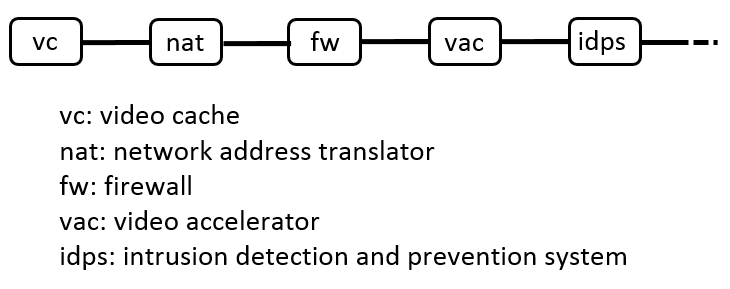
\includegraphics[width=0.9\columnwidth]{example_chain}
  \caption{An example of caching in conjunction with other virtual network functions.}
  \label{fig:example_chain}
\end{figure}
Undoubtedly, among different vNFs, it is expected that caching would emerge as one of the potential key network elements to be supported in emerging and future wireless/mobile networks.  Viral and popular video streams dominate aggregate mobile Internet traffic\footnote{Mobile video traffic accounted for 55 percent of total mobile data traffic in 2015 according to  the CISCO Global Mobile Data Traffic Forecast Update that has been released in February 2016.} and it is an application well suited to various different caching strategies. In that respect, caching of popular content deserves paying a special attention in terms of VNF hosting location and chaining. This is because in the most general case, a cached content must be visited before other VNFs can be applied and this service flow might originate from different possible network locations depending on the caching strategy. Hence, the service does need to reach a gateway node but can originate at a node that host the required cached content (which can be topologically close to the end user). Therefore, the location of caches in a VNF service chain, greatly affects the overall vNF chain orchestration as well as the aggregate traffic dynamics in the network, since links of higher aggregation (deeper in the network) can reduce their utilization levels. However, efficient caching in mobile networks can be deemed as a highly challenging task since the optimality of the cache locations are dependent on the movement/mobility patterns of the users. Notably, to significantly reduce access delays to highly popular content caching content close to the end user without considering the effect of mobility might lead to degradation of performance. In this case, caching popular content closer to the end user might inevitably require more frequently changes of the cache location to keep providing optimal performance. In this case, the caching location and the associated vNF chaining need to be jointly considered to avoid sub-optimal cases, especially under congestion episodes where performance can be significantly affected. To summarize, the focus and motivation of the paper is on enhancing proactive caching  policies by taking into account the whole VNF chain.
\subsection{Motivation and Illustrative Examples}
In this paper, we propose a Proactive caching-chaining (PCC) scheme to enhance the mobility support of SDN-enabled/NFV service chaining in mobile networks. To motivate the research we discuss illustrative examples of the cross issues between caching and VNF chaining that aim to shed further light on some of the key challenges. To start with, Figure \ref{fig:mobility_chain} shows the case of a service with two NF where the first one is caching and the other one is assumed to be a video acceleration network function. As can be seen from the figure, Case I entails a  sub-optimal allocation when mobility is also taken into account. Case II shows a more suitable NF location where after the mobility event the cache and chain location is topologically closer to the end user; in Case II the NFs are located 3 hops away from the end user after the mobility event whereas in Case I, which a mobility oblivious allocation the NFs are located 4 hops away. Figure \ref{fig:noVM} shows the case where VNF chaining and pro-active caching take place independently. The figure shows potential pro-active caching locations but not in all of those pre-selected locations from the caching algorithm it is possible to host the other NFs due to numerous reasons such
as for example reservation policies, placement based on affinity and/or anti-affinity rules and overall resource usage of the virtual machines \cite{affinity_NF}; for example only in one of those locations the two NF can be co-located (node b). Furthermore, as shown in figure \ref{fig:opt_cache_chain} the optimal location of caching and the other NF in the service chain might be different; in the figure shown the optimal location of caching is in node (b) whereas the NF for video acceleration is located at node (d). It is therefore important firstly to consider the issue of caching and service chaining in a holistic integrated manner and secondly to optimize the location and chaining of the different NF in order to increase overall network performance.

Based on the above discussion, the proposed scheme proactively performs caching and VNF chaining so that overall network performance is optimized whilst end user receive their requests seamlessly. Notably, we take VNF chaining allocation and proactive caching as a joint problem and formulate it as a Integer Linear Programming (ILP) problem that minimize the combine cost of VNF placement, chaining and routing. We also investigate the performance obtained of a proposed scale-free heuristic algorithm since the problem resembles the $NP$-hard binpacking optimization problem.

In summary, we hereafter make the following key contributions,
We firstly, propose a novel VNF chaining placement scheme, namely, proactive caching-chaining (PCC) that improves the mobility support for the up coming SDN-enabled/NFV network framework.
Furthermore, we model and formulate the joint proactive caching and chaining problem to obtain optimal routing and placement cost and based on that we devise a scalable heuristic approach and evaluate the performance of the system.
\begin{figure}
  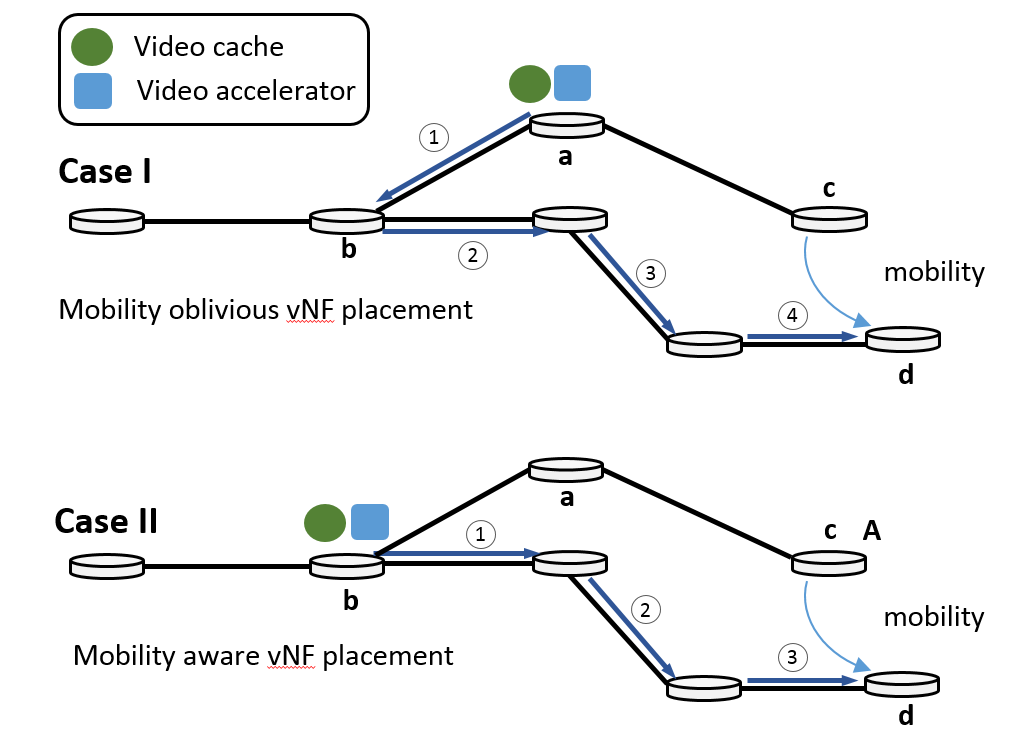
\includegraphics[width=0.9\columnwidth]{cache_mobility}
  \caption{Effect of mobility on the joint caching VNF chaining problem.}
  \label{fig:mobility_chain}
\end{figure}
\begin{figure}
  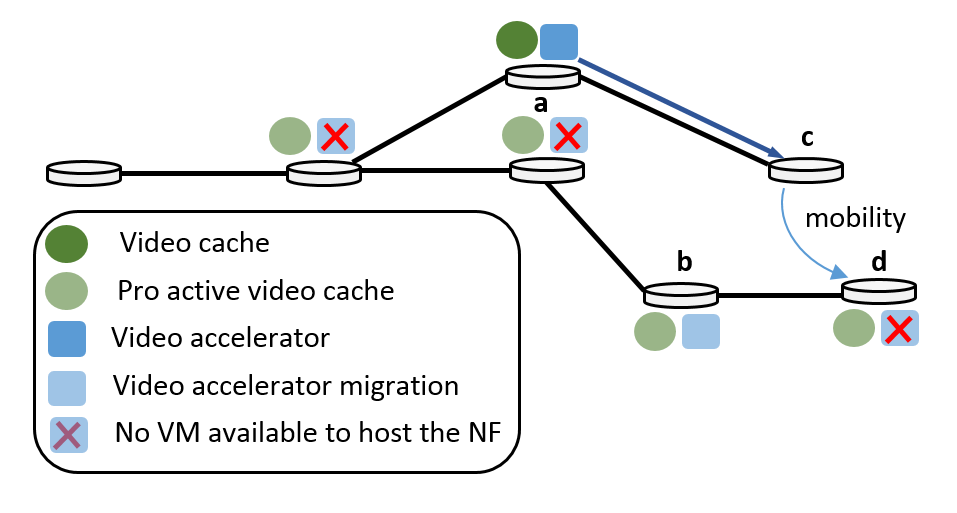
\includegraphics[width=0.9\columnwidth]{no_VM_available}
  \caption{Limited availability of resources (in terms of Virtual Machines for example) in the candidate pro-active caching locations to host the required VNFs for the service.}
  \label{fig:noVM}
\end{figure}
\begin{figure}
  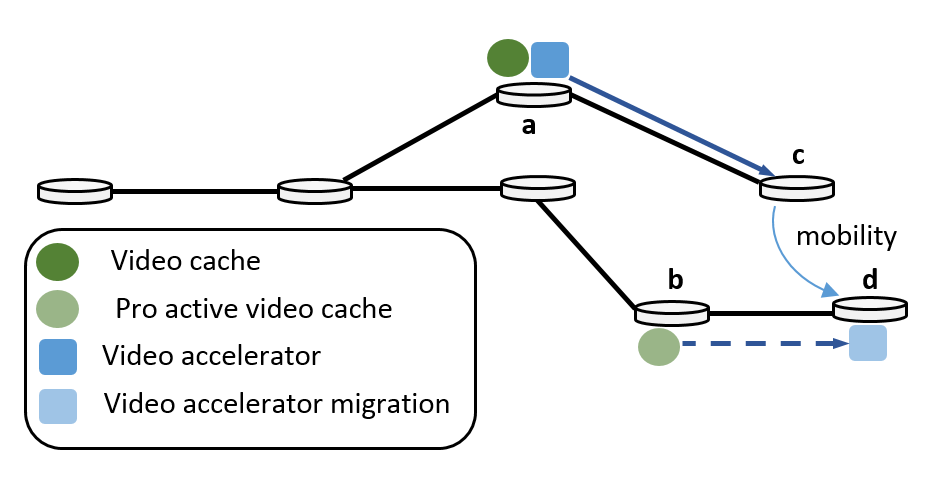
\includegraphics[width=0.9\columnwidth]{cache_chain}
  \caption{An optimal VNF chain NF are located in different nodes in the network.}
  \label{fig:opt_cache_chain}
\end{figure}

\section{Previous Research Work}
The overall logical architecture of the so-called VNF Management and Orchestration (MANO) architecture has been mainly an industry-lead initiative and has been defined within ETSI \cite{NFV}. An example of a VNF orchestrator, which is called \emph{Stratos} is presented in\cite{Stratos} and is built on top of a \emph{Floodlight}\footnote{\texttt{www.projectfloodlight.org}} controller. The work in \cite{Split/Merge} can be considered as another effort to provide orchestration between virtualized NFs especially with  emphasis on issues such as Virtual Machine (VM) migration and split/merging of service flows. An overview of the challenges emerging in virtual network function scheduling is presented in \cite{Riera}; in this paper the authors explain the application of SDN and NFV technologies with emphasis on backbone networks.
In terms of caching there has been recently a significant amount of work. A caching scheme suitable for mobile networks that takes into account user mobility has been proposed in  \cite{op_caching} where the idea is to  predict  the mobility pattern of users and opportunistically cache content along the predicted path of users. A scheme that pro-actively cache content using transportation and focusing on video content has been presented in \cite{caching_transportation}. The idea is to utilize the almost deterministic mobility of users in transportation systems such as trains to proactively cache popular content that the users might request upon their arrival. The ideas on proactive caching in this paper
resemble more closely the work in \cite{PCWR, Efficient proactive caching for support seamless mobility} which propose a set of mobility-aware caching schemes.

However, none of previous research works make caching decisions on a view of the whole service chain. To the best of our knowledge this is the first work to consider in an explicit and integrated manner proactive caching as part of a VNF chain. In most practical cases, this simple cache moving could lead to inefficient routing of a mobile user to receive a service. Fig 1 gives an example of the inefficient routing problem where firewall as a NF must also be visited and only cache is moved \footnote{NF movement in this paper refers to any approach that occurs the change of the function's location. (e.g., proactive caching)}. It is apparent that, in order to improve the mobility support of SDN-enabled networking, other NFs on a same VNF service chain must also be moved, with the decision of caching. A close related work can be found  in \cite{specifying and placing chains of virtual network functions} which aims to assign VNFs into given SDN-enabled networks. However, it does not take routing and location of VNFs into consideration.

%(The work in \cite{Anthony} proposes a VNF placing scheme that addresses this problem, but only wired network scenario is considered.) In fact, caching and VNF chaining should not be treated independently in regard to SDN-enabled networking mobility enhancement. However, to the best of our knowledge, there is little work providing mobility-aware NF allocation for SDN-enabled networking where caching  and VNF chaining are jointly considered.




%\begin{figure*}[!t]

%\centering

%\subfloat[]{\label{fig1}\includegraphics[width=1\columnwidth]{Inefficient_routing_a.pdf}}
%\subfloat[]{\label{fig2}\includegraphics[width=1\columnwidth]{Inefficient_routing_b.pdf}} \\

%\caption{(a) Inefficient routing: only cache is moved;  (b) Optimal: both cache and firewall are moved.}

%\end{figure*}

% The remainder of this paper is organized as follows: In section \uppercase\expandafter{\romannumeral2}, we present our proactive caching with redirection (PCWR) scheme and formulate it into Uncapacitated Optimal Problem (UOP) and Capacitated Optimal Problem (COP). In section \uppercase\expandafter{\romannumeral3}, we show our simulation results and the comparison against other caching solutions. Finally, we give our conclusion in Section \uppercase\expandafter{\romannumeral4} and detail future avenues of research.



%\subsection{Subsection Heading Here}



% needed in second column of first page if using \IEEEpubid
%\IEEEpubidadjcol

% An example of a floating figure using the graphicx package.
% Note that \label must occur AFTER (or within) \caption.
% For figures, \caption should occur after the \includegraphics.
% Note that IEEEtran v1.7 and later has special internal code that
% is designed to preserve the operation of \label within \caption
% even when the captionsoff option is in effect. However, because
% of issues like this, it may be the safest practice to put all your
% \label just after \caption rather than within \caption{}.
%
% Reminder: the ``draftcls'' or ``draftclsnofoot'', not ``draft'', class
% option should be used if it is desired that the figures are to be
% displayed while in draft mode.
%
%\begin{figure}[!t]
%\centering
%\includegraphics[width=2.5in]{myfigure}
% where an .eps filename suffix will be assumed under latex,
% and a .pdf suffix will be assumed for pdflatex; or what has been declared
% via \DeclareGraphicsExtensions.
%\caption{Simulation Results}
%\label{fig_sim}
%\end{figure}

% Note that IEEE typically puts floats only at the top, even when this
% results in a large percentage of a column being occupied by floats.


% An example of a double column floating figure using two subfigures.
% (The subfig.sty package must be loaded for this to work.)
% The subfigure \label commands are set within each subfloat command, the
% \label for the overall figure must come after \caption.
% \hfil must be used as a separator to get equal spacing.
% The subfigure.sty package works much the same way, except \subfigure is
% used instead of \subfloat.
%
%\begin{figure*}[!t]
%\centerline{\subfloat[Case I]\includegraphics[width=2.5in]{subfigcase1}%
%\label{fig_first_case}}
%\hfil
%\subfloat[Case II]{\includegraphics[width=2.5in]{subfigcase2}%
%\label{fig_second_case}}}
%\caption{Simulation results}
%\label{fig_sim}
%\end{figure*}
%
% Note that often IEEE papers with subfigures do not employ subfigure
% captions (using the optional argument to \subfloat), but instead will
% reference/describe all of them (a), (b), etc., within the main caption.


% An example of a floating table. Note that, for IEEE style tables, the
% \caption command should come BEFORE the table. Table text will default to
% \footnotesize as IEEE normally uses this smaller font for tables.
% The \label must come after \caption as always.
%
%\begin{table}[!t]
%% increase table row spacing, adjust to taste
%\renewcommand{\arraystretch}{1.3}
% if using array.sty, it might be a good idea to tweak the value of
% \extrarowheight as needed to properly center the text within the cells
%\caption{An Example of a Table}
%\label{table_example}
%\centering
%% Some packages, such as MDW tools, offer better commands for making tables
%% than the plain LaTeX2e tabular which is used here.
%\begin{tabular}{|c||c|}
%\hline
%One & Two\\
%\hline
%Three & Four\\
%\hline
%\end{tabular}
%\end{table}


% Note that IEEE does not put floats in the very first column - or typically
% anywhere on the first page for that matter. Also, in-text middle (``here'')
% positioning is not used. Most IEEE journals use top floats exclusively.
% Note that, LaTeX2e, unlike IEEE journals, places footnotes above bottom
% floats. This can be corrected via the \fnbelowfloat command of the
% stfloats package.

\section{Network Modeling and Proactive chaining with caching}

%\begin{figure}
%\includegraphics[width=1\columnwidth]{Proactive_caching_chaining.pdf}
%\caption{Proactive caching-chaining}
%\end{figure}
A mobile network is modeled as an undirected  graph $G=(N,E)$, where $\mathbf{N}$ denotes the set of nodes in the network and $E$ denotes the set of links in the network. By $\mathbf{F}$, we denote the set of NFs and $f_{i}$ represents the specific NF$_{i}$. Each $f_{i}$, if activated, consumes/requires some physical resources (i.e., CPU cycles, DRAM memory). We uniformly describe these resource requirements as a single column matrix $u_{i}$, meanwhile, the amount of available resources of node $k$, which is able to host VNFs, is denoted using the single column matrix $U_{k}$.

The term ``chain'' in the so-called service chaining represents the different middleboxes that the service should traverse, with a specific order, across the network using software provisioning. This is the case under the proposed NFV architecture, where new services and/or network slices can be instantiated as software-only, running on commodity hardware on top of virtual machines or containers. To provide a service request $r\in \mathbf{R}$ (with $\mathbf{R}$ we denote the set of requests) for a mobile user and/or tenant, a network function forwarding graph (VNF-FG)\cite{VNF-FG} needs to access a set of corresponding NFs that are visited in a pre-defined order (which the VNF orchrstrator should preserve). In this paper, we consider the form of service request $r$ as the set $r=\{f_{1}, f_{2}, \cdots, f_{i}\}$ where the sequence express the visiting order of the different network functions. For modeling simplification reasons the corresponding relationship of a NF and its order in a request, can be represented by a binary matrix $V_{ril}$, as follows,

\begin{equation}
  V_{ril} = \left \{
  \begin{array}{rl}
    1 & \text{if the $l^{th}$ NF of request $r$ is NF$_{i}$}. \\
    0 & \text{otherwise}.
  \end{array} \right.
\end{equation}

Hereafter, we consider the scenario where a mobile user and/or tenant connected to node $o$ and requesting $\mathbf{R}$ services. As presented in Figure 2, caching as a NF, is the head of a service request chain and it is denoted as $f_{0}$. We define a candidate node set $\mathbf{K}\subseteq \mathbf{N}$ that consist of the potential candidate nodes of hosting NFs. By $\mathbf{D}$, we define a set of potential destinations that mobile users might move due to their inherent mobility. Using historical data available to mobile network providers it is feasible to  estimate such probabilities of end users moving from their current  location to an a adjacent candidate destination node $d$. We denote this probability of changing their serving access router with $\rho_{d}$. As eluded, we assume that $\rho_{d}$ is predefined by using available historical data from operators so this assumption can be deemed as realistic due to vast available data which can provide accurate  characterization of user mobility patterns. With known candidate cache locations, which can be done using for example a proactive caching technique such as PCWR\cite{PCWR}), PCC aims to proactively place network functions $f_{i}\in \mathbf{F}$ into the set of nodes $\mathbf{K}$. To be more precise, we define by $\mathbf{S_{r}}$ to be the set of initiating nodes (i.e., proactive caching locations) of a service chain $r$, with  $\mathbf{H}$ denoting the set of $\mathbf{S_{r}}$. Given $\mathbf{H}$ and $\mathbf{D}$, the proposed scheme returns the optimal proactive allocation of the NFs that minimizes the joint cost of routing, location and chaining.


\subsection{Proactive chaining-caching problem}
Based on the previously described network settings we define the following binary decision variables,

\begin{equation}
  x_{i} ^{k} = \left \{
  \begin{array}{rl}
    1 & \text{if NF$_{i }$ is placed at $k$}. \\
    0 & \text{otherwise}.
  \end{array} \right.
\end{equation}

\begin{equation}
  y_{ri} ^{ksd} = \left \{
  \begin{array}{rl}
    1 & \text{if NF$_{i}$ of request $r$ with head $s$ and} \\
    &\text{destination $d$ is visited from $k$}. \\
    0 & \text{otherwise}.
  \end{array} \right.
\end{equation}

The optimal proactive chaining-caching problem is defined as the following non-linear integer optimization problem,


\begin{equation}
  \begin{split}
    %\label{eq:objective1}
    \underset{x_{i}^{k},y_{ri}^{ksd}}{\min} \: \sum_{k \in \mathbf{K}}\sum_{i \in \mathbf{F}} C_{i}^{k} x_{i}^{k}+\sum_{r \in \mathbf{R}}\sum_{s \in \mathbf{S_{r}}}\sum_{d \in \mathbf{D}} \sum_{k \in \mathbf{K}}\sum_{i \in \mathbf{F}} \rho_{d} P_{sk} V_{ri1} y_{ri}^{ksd}+ \\ \sum_{r \in \mathbf{R}}\sum_{s \in \mathbf{S_{r}}}\sum_{d \in \mathbf{D}}\sum_{k,m \in \mathbf{K}}\sum_{i,j \in \mathbf{F}} \sum_{l=1}^{L-1} \rho_{d} P_{km}V_{ril} y_{ri}^{ksd}V_{rj(l+1)} y_{rj}^{msd} +\\ \sum_{r \in \mathbf{R}}\sum_{s \in \mathbf{S_{r}}}\sum_{d \in \mathbf{D}}\sum_{k \in \mathbf{K}}\sum_{i \in \mathbf{F}} \rho_{d} P_{kd} V_{riL} y_{ri}^{ksd}
  \end{split}
\end{equation}
\label{eq:con1}
\begin{IEEEeqnarray}{cl}
  \text{S.t.} \: \:
  %\label{eq:con1}
  \sum_{i \in \mathbf{F}}  u_{i} x_{i}^{k} \leq U_{k} , \forall k \in \mathbf{K} \IEEEyessubnumber \\
  \label{eq:con2}
  \sum_{k \in \mathbf{K}}\sum_{i \in \mathbf{F}}V_{ril}y_{ri}^{ksd} \geq 1, \: \forall r \in \mathbf{R}, s \in \mathbf{S_{r}}, d \in \mathbf{D}, \nonumber \\l=1, \ldots L  \IEEEyessubnumber \\
  \label{eq:con3}
  x_{i}^{k}-y_{ri}^{ksd} \leq 0, \forall r\in \mathbf{R}, i\in \mathbf{F}, k \in \mathbf{K}, s \in \mathbf{S_{r}}, d \in \mathbf{D} \IEEEyessubnumber \\
  \label{eq:con4}
  x_{i}^{k} \in \{0,1\}, \:\:\: \forall i \in \mathbf{F}, k \in \mathbf{K}\IEEEyessubnumber \\
  \label{eq:con5}
  y_{ri}^{ksd} \in \{0,1\}, \:\:\: \forall r \in \mathbf{R}, i \in \mathbf{F}, k \in \mathbf{K}, s \in \mathbf{S_{r}}, d \in \mathbf{D} \IEEEyessubnumber
\end{IEEEeqnarray}
where $C_{i}^{k}$ is the cost of placing NF$_{i}$ at $k$. While $P_{sk}$, $P_{km}$ and $P_{kd}$ are the shortest path routing costs between the candidate nodes. Constraint (4a) bounds the resources that can be consumed by each NF in every node. (4b) enforce that each NF in a requested chain must be visited at least once. (4C) is a binding constraint that insures the availability of a NF at a node is valid only when the NF is hosted at the node.

The first term of the objective function is the placement cost of hosting VNFs at a node. The rest of the terms in the objective function reflect the accumulative routing cost of each hop on the VNF-FG of a requested chain. To linearize the optimization problem, we replace the product of binary decision variables $y_{ri}^{ksd}y_{rj}^{msd}$ with an auxiliary variable $z_{rij}^{kmsd}$, which is defined as follows,

\begin{equation}
  z_{rij} ^{kmsd} = \left \{
  \begin{array}{rl}
    1 & \text{if request $r$ with head $s$ and destination $d$} \\
    &\text{visits NF$_i$ at node $k$ and NF$_j$ at node $m$}. \\
    0 & \text{otherwise}.
  \end{array} \right.
\end{equation}

Hereafter, the optimization problem is converted to the integer linear programming problem shown as follows,

\begin{equation}
  \begin{split}
    %\label{eq:objective1}
    \underset{x_{i}^{k},y_{ri}^{ksd}}{\min} \: \sum_{k \in \mathbf{K}}\sum_{i \in \mathbf{F}} C_{i}^{k} x_{i}^{k}+\sum_{r \in \mathbf{R}}\sum_{s \in \mathbf{S_{r}}}\sum_{d \in \mathbf{D}} \sum_{k \in \mathbf{K}}\sum_{i \in \mathbf{F}} \rho_{d} P_{sk} V_{ri1} y_{ri}^{ksd}+ \\ \sum_{r \in \mathbf{R}}\sum_{s \in \mathbf{S_{r}}}\sum_{d \in \mathbf{D}}\sum_{k,m \in \mathbf{K}}\sum_{i,j \in \mathbf{F}} \sum_{l=1}^{L-1} \rho_{d} P_{km}V_{ril} V_{rj(l+1)} z_{rij}^{kmsd} +\\ \sum_{r \in \mathbf{R}}\sum_{s \in \mathbf{S_{r}}}\sum_{d \in \mathbf{D}}\sum_{k \in \mathbf{K}}\sum_{i \in \mathbf{F}} \rho_{d} P_{kd} V_{riL} y_{ri}^{ksd}
  \end{split}
\end{equation}
\label{eq:con1}
\begin{IEEEeqnarray}{cl}
  \text{S.t.} \: \:
  %\label{eq:con1}
  \sum_{i \in \mathbf{F}}  u_{i} x_{i}^{k} \leq U_{k} , \forall k \in \mathbf{K} \IEEEyessubnumber \\
  \label{eq:con2}
  \sum_{k \in \mathbf{K}}\sum_{i \in \mathbf{F}}V_{ril}y_{ri}^{ksd} \geq 1, \: \forall r \in \mathbf{R}, s \in \mathbf{S_{r}}, d \in \mathbf{D}, \nonumber \\l=1, \ldots L  \IEEEyessubnumber \\
  \label{eq:con3}
  x_{i}^{k}-y_{ri}^{ksd} \leq 0, \forall r\in \mathbf{R}, i\in \mathbf{F}, k \in \mathbf{K}, s \in \mathbf{S_{r}}, d \in \mathbf{D} \IEEEyessubnumber \\
  \label{eq:con4}
  z_{rij}^{kmsd} \leq y_{ri}^{ksd}, \forall r\in \mathbf{R}, i\in \mathbf{F}, k \in \mathbf{K}, s \in \mathbf{S_{r}}, d \in \mathbf{D} \IEEEyessubnumber \\
  \label{eq:con5}
  z_{rij}^{kmsd} \leq y_{rj}^{msd}, \forall r\in \mathbf{R}, i\in \mathbf{F}, k \in \mathbf{K}, s \in \mathbf{S_{r}}, d \in \mathbf{D} \IEEEyessubnumber \\
  \label{eq:con6}
  z_{rij}^{kmsd} \geq y_{ri}^{ksd}+y_{rj}^{msd}-1, \forall r\in \mathbf{R}, i\in \mathbf{F}, k \in \mathbf{K}, \nonumber \\ s \in \mathbf{S_{r}}, d \in \mathbf{D} \IEEEyessubnumber \\
  \label{eq:con7}
  x_{i}^{k} \in \{0,1\}, \:\:\: \forall i \in \mathbf{F}, k \in \mathbf{K}\IEEEyessubnumber \\
  \label{eq:con8}
  y_{ri}^{ksd} \in \{0,1\}, \:\:\: \forall r \in \mathbf{R}, i \in \mathbf{F}, k \in \mathbf{K}, s \in \mathbf{S_{r}}, d \in \mathbf{D} \IEEEyessubnumber \\
  \label{eq:con9}
  z_{rij}^{kmsd} \in \{0,1\}, \:\:\: \forall r \in \mathbf{R}, i \in \mathbf{F}, k \in \mathbf{K}, s \in \mathbf{S_{r}}, d \in \mathbf{D} \IEEEyessubnumber
\end{IEEEeqnarray}

where (6d)-(6f) are binding constraints that insure $z_{rij}^{kmsd}$ taking the same value as product $y_{ri}^{ksd}y_{rj}^{msd}$.

\section{A Scale Free Heuristic Approach}
The PCC problem falls within the family of $\mathcal{NP}$-hard problems since it resemples a binpacking problem and as a result heuristics, becomes the only viable option of finding competitive feasible solutions for real time operation. Therefore, a heuristics algorithm named, Probability-prior proactive caching-chaining (P-PCC) is proposed and is detailed in the pseudocode Algorithm \uppercase\expandafter{\romannumeral1} below. The main philosophy of the proposed P-PCC heuristic is to create a set of candidate pro-active caching points for each possible visited access router and then weighted by the probability of visiting each access router and explore node combinations for creating the service chain.

\begin{enumerate}%[leftmargin=*]
\item For any request $r$, select the target node $d\in\mathbf{D}$ by highest $\rho_{d}$
  and find the closest starting node $s\in \mathbf{S_{r}}$ by minimum shortest path routing cost $P_{sd}$;
\item On the shortest path from the selected $s$ and $d$, find all candidate nodes by $\mathbf{K}$;
\item Choose the closest $k$ from the selected $s$ on the path to host the NF$_{i}$ with the lowest visiting order sequence in request $r$ if there are enough resources to support the function, otherwise, host the sub-lowest function, until running out of resources;
\item Repeat step 2 and 3 until all NFs of request $r$ are hosted.
\end{enumerate}

\begin{algorithm}
  \caption{P-PCC}
  \SetKwInOut{Input}{Input}
  \SetKwInOut{Output}{Output}
  \Input{$\mathbf{G}$; $\mathbf{D}$; $\mathbf{R}$; $\mathbf{K}$; $\mathbf{F}$; $\mathbf{H}$; attaching node $o$;}
  \Output{VNF allocation: $x_{i}^{k}$; P-PCC cost: P-PCC;}
  P-PCC$\leftarrow 0$\;
  \For{$k \in \mathbf{K}$}{
    Remaining utility of node $k$: $RU_{k} \leftarrow U_{k}$\;
  }

  :// VNF Allocation\\
  \For{$i\in \mathbf{D}$}{
    \If{$\rho_{i}==max(\rho_{i})$}{
      Destination node: $d\leftarrow i$\;
    }
  }
  \For{$r\in \mathbf{R}$}{
    Starting node:$s \leftarrow$ find closest node s to d in $S_{r}$ with minimum $P_{sd}$\;
    candidate node priority list: $CPL \leftarrow \emptyset$\;
    $CPL \leftarrow $ sort $k\in$ \big\{ \{$n\vert n$ is on the shortest path from s to d\} $\cap$ $\mathbf{K}$ \big\} by the distance between $k$ and $s$ from low to high\;
    VNF priority list: $FPL \leftarrow \emptyset$\;
    $FPL \leftarrow $ sort $f_{i}$ by its visiting sequence $l$ of $r$\;
    \For{$k\in CPL$}{
      \For{$f_{i}$ $\in FPL$}{
        \If{$u_{i} \leq RU_{k}$ and $f_{i}$ is not hosted at $k$}{
          host $f_{i}$ at $k$ \;
          $x_{i}^{k} \leftarrow 1$ \;
          label $f_{i}$ as hosted at $k$ \;
          $RU_{k} \leftarrow RU_{k}-u_{i}$\;
          P-PCC $\leftarrow$ P-PCC$+C_{i}^{k}$\;
        }
      }
    }
  }
  $x_{i}^{k}$
  :// Chaining Routing cost\\
  \For{$d\in \mathbf{D}$}{
    \For{$r\in \mathbf{R}$}{
      Length of the chain requested by $r$: $L_{r} \leftarrow$ the number of requested VNFs by $r$\;
      VNF chaining list: $I \leftarrow$ sort $f_{i}$ by its visiting sequence $l$ of $r$\;
      Chaining Routing cost between $I(j)$ and $I(j+1)$: $CR_{j,j+1} \leftarrow$ cumulative $P_{km}$ where $k$ hosts $I(j)$ and $m$ host $I(j+1)$ which is given by $x_{i}^{k}$\;
      Chaining Routing Cost: $CRC\leftarrow 0$\;
      $CRC\leftarrow$ find the cost of shortest chaining routing path from $I(0)$ to $d$\;
      P-PCC$\leftarrow$ P-PCC$+\rho_{d}CRC$\;
    }
  }
  P-PCC\;

\end{algorithm}


\section{Numerical Investigations}
In this section, we provide a wide set of numerical investigations to evaluate the performance of proactive chaining-caching problem under various network scenarios. The applied random networks are composed by an range of 10 to 20 candidate VNF hosting nodes and each candidate node has its degree ranged from 2 to 5. Besides, the number of starting points and destination points are set from 1 to 5. We assume that, the number of requests to be supported is 20, and the number of different VNFs is randomly selected from 1 to 3.

The moving probability to each destination node is randomly generated between 0 and 1, notice that, the summation of the moving probability to each destination of a mobile user does not exceed 1. The shortest path routing cost and the VNF placement cost are measured by general network metrics in the open interval of (0, 100]. In terms of physical resources of candidate VNF hosting node, we assume that each candidate node has 2 GByte memory capacity and 16 virtual CPU cores. While each VNF consumes memory in a range from 10 to 50 MByte and use 0.5 to 1 cores.  The results are obtained by averaging 1000 Monte Carlo simulations. To sum up, the parameters that have been used in the investigations are presented in Table \uppercase\expandafter{\romannumeral1}.


  \begin{table}[h]
    \caption{Simulation Parameters}
    \label{table1}
    \begin{center}
      \begin{tabular}{@{}lc@{}}
        \toprule
        \multicolumn{1}{c}{Parameter}                     & value      \\ \midrule
        Number of candidate hosting nodes($K$)            & 10-20        \\
        Degree per node                                   & 2-5        \\
        Moving probability ($\rho_{d}$)                   & 0-1        \\
        Number of starting points per request ($\mathbf{S_{r}}$)        & 1-5        \\
        Number of destination points per user ($\mathbf{D}$)            & 1-5        \\
        Number of requests to support ($R$)               &20         \\
        VNF number ($F$)                                  & 1-3         \\
        Maximum number of VNF in a chain ($L$)            & 1-3         \\
        Cost metric per link ($P_{km}$)                   & (0,100]      \\
          Cost metric per node to host VNF($C_{i}^{k}$)     & (0,100]      \\
            Memory capacity per candidate node                & 2 GByte     \\
            Number of virtual CPU cores per candidate node    & 16         \\
            Memory requirement per VNF                        & 10-50 MByte \\
            CPU core requirement per VNF                      & 0.5-1        \\

            \\ \bottomrule

      \end{tabular}
    \end{center}
  \end{table}
  \begin{figure}
    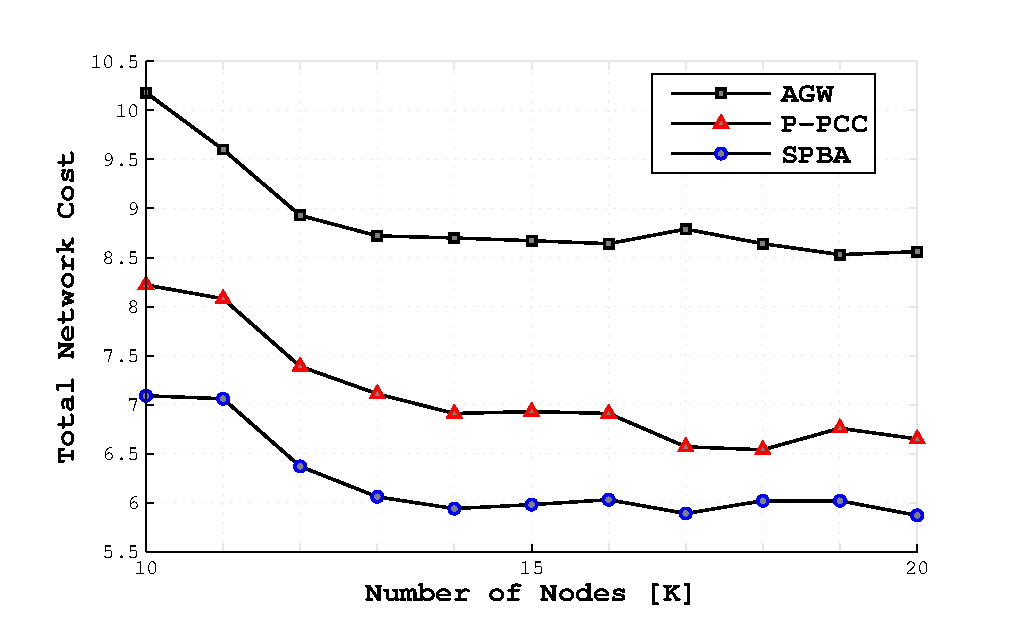
\includegraphics[width=1.1\columnwidth,trim=1.1cm 0.5cm 0cm 0.8cm]{mc_ppcc_naive_K_1020_final.eps}
    %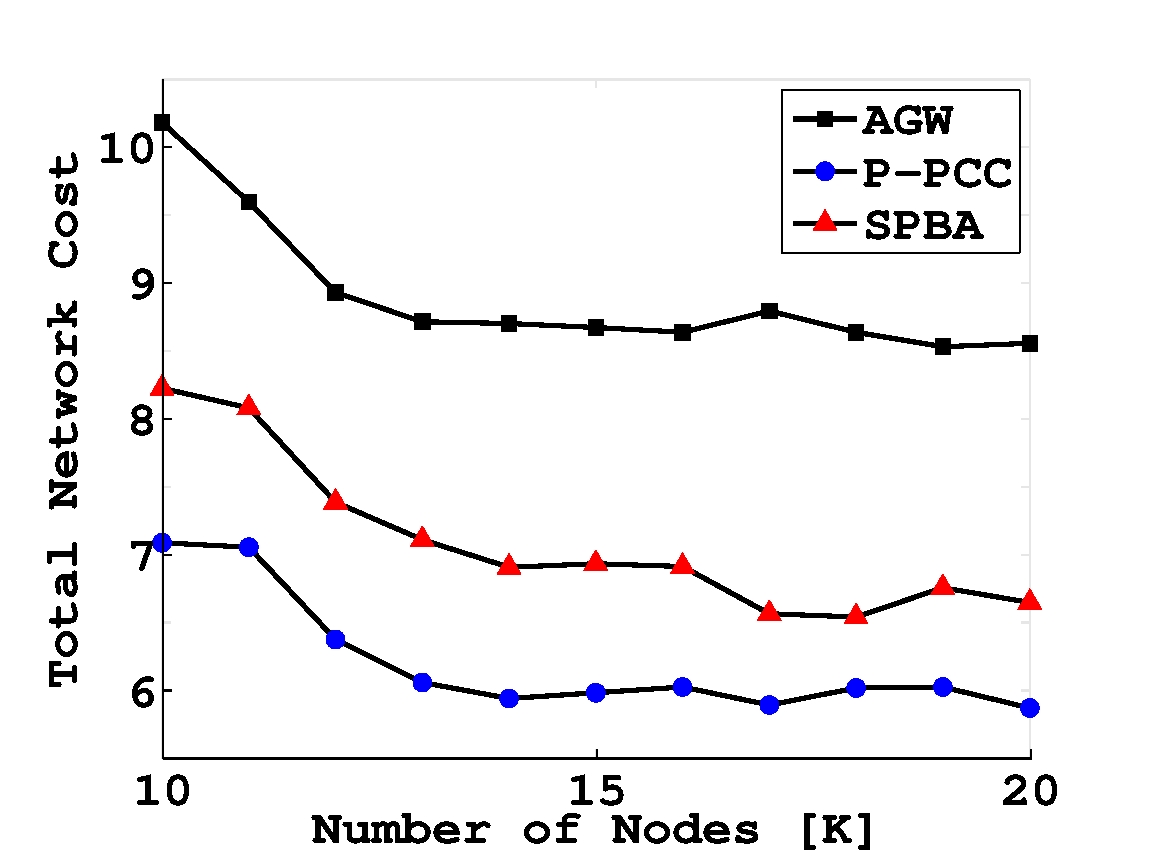
\includegraphics[width=0.85\columnwidth]{cost_no_nodes}
    \caption{Performance of the proposed scheme with different number of nodes in the network.}
    \label{fig:cost_no_nodes}
  \end{figure}
  The proposed scheme is compared with two baseline schemes. In the first one, which provide a lower bound on the performance, content caching and VNFs are hosted at the network gateway, namely, AGW. The second scheme allocates caching as well as VNFs along the shortest path from the gateway node to the serving access router without considering mobility, and is called Shortest Path Based Allocation (SPBA). Figure \ref{fig:cost_no_nodes} shows the performance of the proposed scheme compared to the previous mentioned baseline techniques for different number of nodes in the network. As can be seen from the figure a significant performance gain of over $12\%$ can be achieved which is robust against different network sizes. A similar observation can be made from figure \ref{fig:cost_no_requests}, which shows the performance for different number of requests. With increased  number of requests, i.e., more constrained allocations, the performance gains increase from $4.8\%$ to $8.3\%$. Finally, in figure \ref{fig:cost_mobility} we show the performance of the proposed scheme for different mobility use cases. The figure shows the performance gains as a factor of the parameter $\rho_{o}$. This parameter is defined as follows $\rho_{o} = 1 -  \sum_{d \in \mathbf{D}} \rho_d$, which means that as $\rho_{o}$ reaches close to 1 there is no mobility of the end-user, i.e., there is no change on the serving access router. As expected, there are no gains when there is no mobility, but as the mobility increase the gains reach up to $15\%$.


  % The PCC performance is investigated along with the proposed heuristics as well as the basic scheme where no optimization applies. We use the ``Intlinprog'' solver (i.e. Mixed Integer Linear Programming solver provider by MathWorks) to calculate the optimal value of our optimization problem. The results are obtained by averaging 1000 Monte Carlo simulations. Figure 3 shows the cost distributions by different schemes. As can be seen, PCC in general achieves $ [x]\%$ lower network cost against the non-optimization scheme. On the other hand, P-PCC as a heuristic, sacrifices $[x]\%$ cost performance for computation time. To further evaluate the performance of the proposed scheme under different network scenarios, Figure 4 presents the cost curve by the change of network size. Within the tested range, the cost curve of PCC grows more smooth than the one of P-PCC. And the error gap between the two schemes increases dramatically when the network size goes huge. However, both PCC and P-PCC receives consistent significant gains of over $[x]\%$ against the non-optimization scheme. Figure 5 returns the results showing the scalability of request size of the three schemes, which suggests that PCC has the best scalability performance with the increasing demand of request service. P-PCC in general, has $[x]\%$ higher cost than PCC, however,
  \begin{figure}
    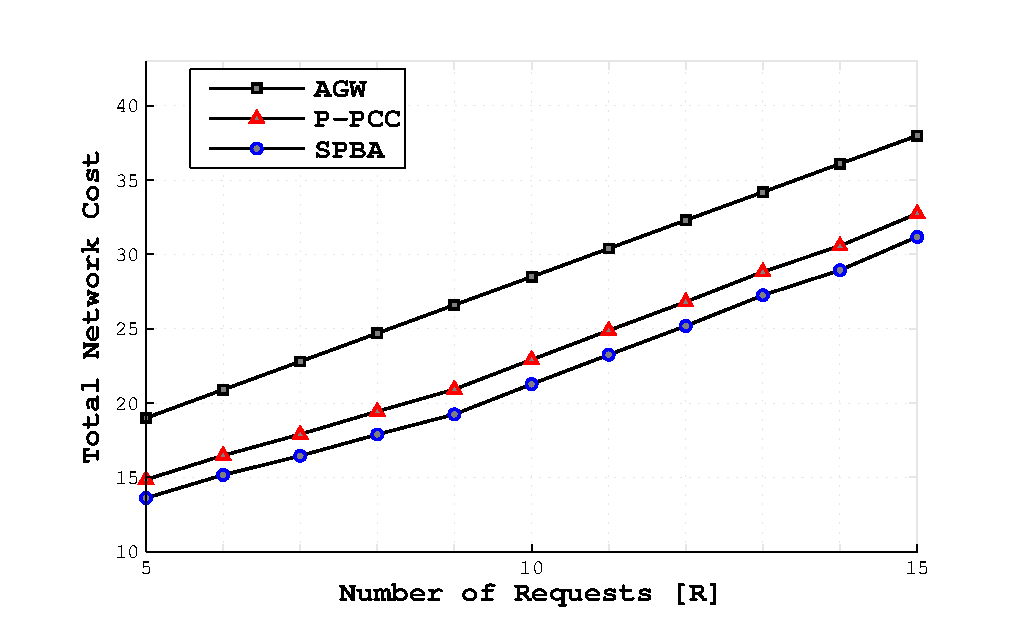
\includegraphics[width=1.1\columnwidth,trim=1.1cm 0.5cm 0cm 0.8cm]{mc_ppcc_naive_R_520_final.eps}
    %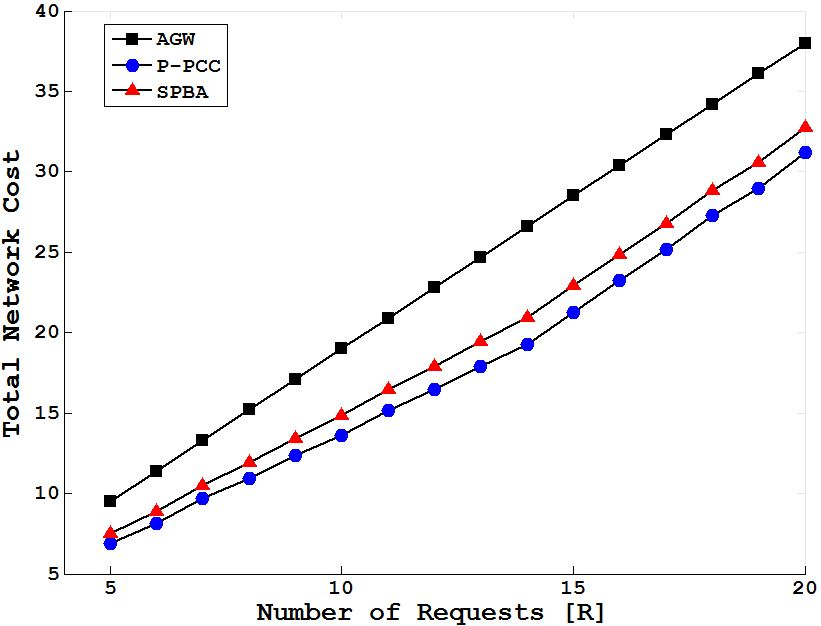
\includegraphics[width=0.85\columnwidth]{cost_no_request}
    \caption{Performance of the proposed scheme with increased number of service requests in the network.}
    \label{fig:cost_no_requests}
  \end{figure}
  \begin{figure}
    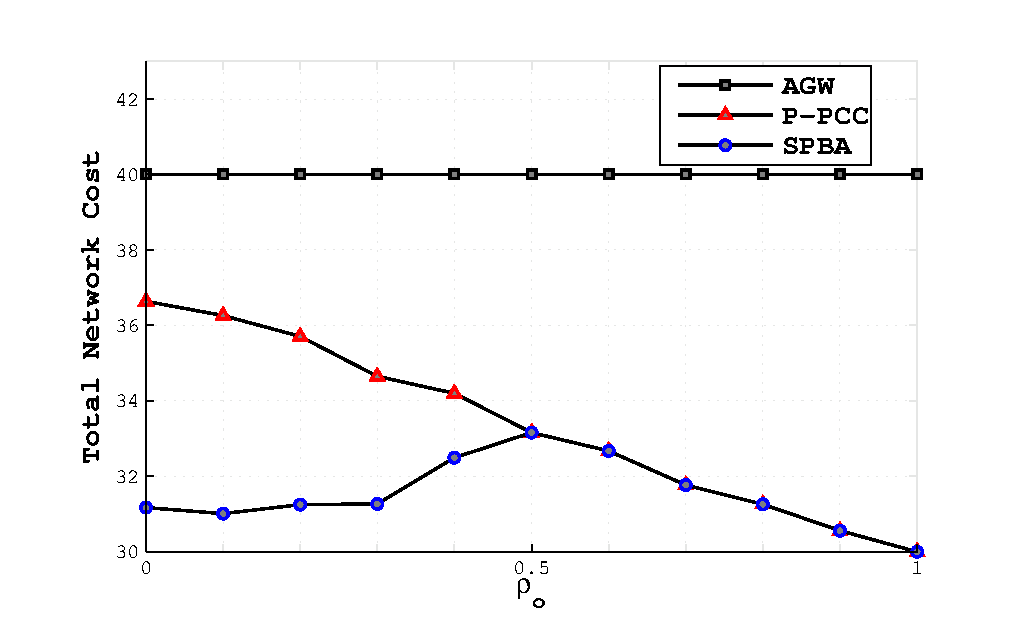
\includegraphics[width=1.1\columnwidth,trim=1.1cm 0.5cm 0cm 0.8cm]{mc_ppcc_naive_static_Rho_0_100_final.eps}
    %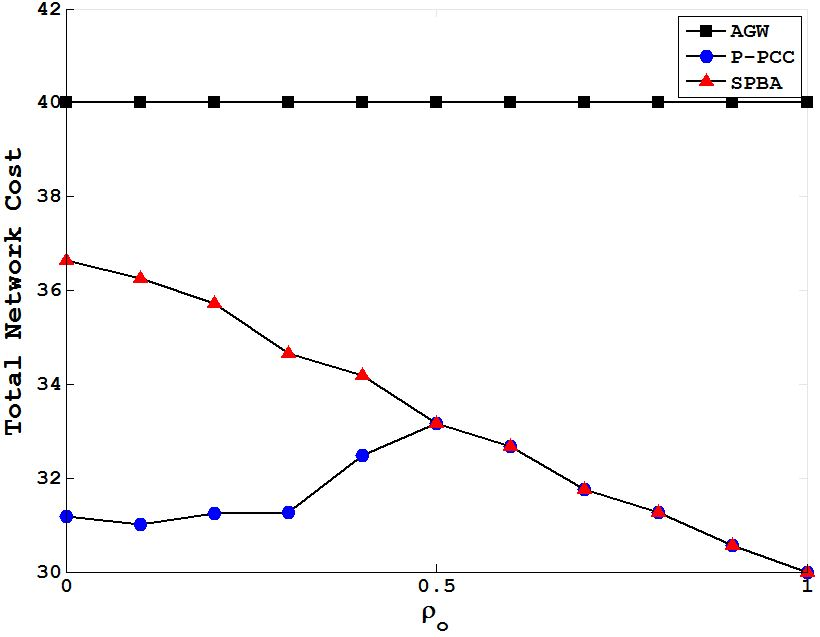
\includegraphics[width=0.85\columnwidth]{cost_mobility}
    \caption{Performance of the proposed scheme for different values of the parameter $\rho_0$.}
    \label{fig:cost_mobility}
  \end{figure}
  \section{Conclusions}
  In this paper, the rational of joint proactive caching and VNF chaining has been presented together with some key observations on this problem and the general principle of optimizing cache specific VNF service chains. Based on those preliminaries an optimization framework using integer linear mathematical programming has been detailed that integrates VNF chaining with proactive caching. In addition, since the problem resembles the multi-dimensional binpacking problem, which is $NP$-hard, a scale-free heuristic algorithm has been presented that can be applied in large network instances amenable for real time implementations. Finally, the attainable
  performance of the proposed proactive caching service chains schemes was investigated.

  %%%%%%%%%%%%%%%%%%%%%%%%%%%%%%%%
  %%                            %%
  %%      ACKNOLEDGEMENTS       %%
  %%                            %%
  %%%%%%%%%%%%%%%%%%%%%%%%%%%%%%%%
  \section*{Acknowledgment}
  This work has been performed in the framework of H2020-ICT-2014-2 project 5G NORMA. The authors would like to acknowledge the contributions of their colleagues, although the views expressed are those of the authors and do not necessarily represent the project.
  % This information reflects the consortium's view, but the consortium is not liable for any use that may be made of any of the information contained therein.
  %\\


  %%%%%%%%%%%%%%%%%%%%%%%%%%%%%%%%
  %\textbf{References}
  \begin{thebibliography}{1}

  \bibitem{VNF state of art}
    R. Mijumbi et al., ``Network function virtualization: State-of-the-art and
    research challenges,'' \emph{IEEE Commun. Surveys Tuts}., Vol. 18, No. 1, 2016
  \bibitem{NFV}
    Network Function Virtualisation: ETSI introductory white paper,
    \text{http://portal.etsi.org/NFV/NFV\_White\_Paper.pdf}, October 2012.
  \bibitem{Stratos}
    Gember A., Krishnamurthy A., Saul St. John, Grandl R, Gao X., Anand A, Benson T., Sekar V., Akella A. (2013), Stratos: A Network-Aware Orchestration Layer for Virtual Middleboxes in Clouds, Technical Report, 2013
  \bibitem{Split/Merge}
    Rajagopalan S., Williams D., Jamjoom H., Warfield A., Split/Merge: System Support for Elastic Execution in Virtual Middleboxes, ACM USENIX Symposium on Networked Systems Design and Implementation, 2013
  \bibitem{Riera}
    Riera F., et al., On the complex scheduling formulation of virtual network functions over optical networks, 16th International Conference on Transparent Optical Networks (ICTON), 2014
  \bibitem{op_caching}
    T.   Han   and   N.   Ansari,   Opport
    unistic   content   pushing   via   WiFi hotspots, in
    Proc. 3rd IEEE IC-NIDC, Sep. 2012, pp. 680–684
  \bibitem{caching_transportation}
    K. Kanai et al., Proactive Content Caching for Mobile Video Utilizing Transportation Systems and Evaluation Through Field Experiments, in IEEE Journal on Selected Areas in Communications, vol. 34, no. 8, pp. 2102-2114, Aug. 2016.

  \bibitem{NFV_overview}
    R. Guerzoni, ``Network Functions Virtualisation: An Introduction, Benefits,  Enablers,  Challenges  and  Call  for  Action.  Introductory  white paper'', in \emph{Proc. SDN and OpenFlow World Congress}, Jun. 2012 pp. 1-16.
    % \bibitem{5GNORMA}
    % EU-HORIZON 2020 5G-PPP 5G NORMA research project, \text{wwww.5gnorma.5g-ppp.eu}, 2015

  \bibitem{affinity_NF}
    S. Lee, S. Pack,  M-K. Shin, E. Paik, R. Browne, Resource Management in Service Chaining, Internet Research Task Force (IRTF), Internet-Draft, July 2015

  \bibitem{Scalable and Flexible cellular core network Architecture}
    X. Jin, L. Erran Li, L. Vanbever and J. Rexford, ``SoftCell: Scalable and flexible cellular core network architecture'', \emph{Proc. 9th Int. Conf. Emerging Netw. Exp. Technol}., pp. 163-174, 2013.
  \bibitem{SDN}
    O. N. Fundation, ``Software-defined networking: The new norm for networks,'' \emph{ONF White Paper}, 2012.
  \bibitem{VNF Chaining basic}
    ``ETSI GS NFV 002 V1.2.1: Network Functions Virtualisation (NFV);
    Architectural framework,'' ETSI Ind. Spec. Group (ISG) Netw. Functions
    Virtualisation (NFV), Sophia-Antipolis Cedex, France, Dec. 2014.
    [Online]. Available: \text{http://www.etsi.org/deliver/etsi\_gs/NFV/001\_099/}
    \text{002/01.02.01\_60/gs\_NFV002v010201p.pdf}
  \bibitem{ICN basic}
    G. Xylomenos, C. Ververidis, V. Siris, N. Fotiou, C. Tsilopoulos, X. Vasilakos, K. Katsaros, and G. Polyzos, ``A Survey of Information-Centric Networking Research'', in \emph{IEEE Commun. Surv. Tut}. (available online since 19 July 2013).
  \bibitem{cache in the air}
    X. Wang, ``Cache in the Air: Exploiting Content Caching and Delivery Techniques for 5G Systems'', \emph{IEEE Commun. Mag}., vol. 52, no. 2, pp. 131-39.
  \bibitem{PCWR}
    G. Zheng, V. Friderikos, ``Optimal proactive caching management in mobile networks'' in \emph{Proc. IEEE ICC}, 2016.
  \bibitem{Efficient proactive caching for support seamless mobility}
    V. A. Siris, X. Vasilakos, and G. C. Polyzos, ``Efficient proactive caching for supporting seamless mobility,'' \emph{arXiv preprint arXiv}:1404.4754, 2014.
  \bibitem{specifying and placing chains of virtual network functions}
    S. Mehraghdam, M. Keller, and H. Karl, ``Specifying and placing chains of virtual network functions,'' in \emph{Proc. IEEE 3rd Int. Conf. CloudNet}, Oct. 2014, pp. 7-13.
  \bibitem{VNF-FG}
    ``ETSI GS NFV 001 V1.1.1: Network Functions Virtualisation (NFV);
    Use Cases,'' ETSI Ind. Spec. Group (ISG) Netw. Functions
    Virtualisation (NFV), Sophia-Antipolis Cedex, France, Oct. 2013.
    [Online]. Available: \text{http://www.etsi.org/deliver/etsi\_gs/nfv/001\_099/}
    \text{001/01.01.01\_60/gs\_nfv001v010101p.pdf}
  \end{thebibliography}
  % that's all folks
\end{document}


